\documentclass{article}
\usepackage[utf8]{inputenc}
\usepackage{siunitx}
\usepackage{graphics}
\usepackage[american,siunitx]{circuitikz}
\usepackage{amsmath}
\usepackage{svg}
\usepackage{booktabs}
\usepackage{float}
\usepackage{xparse, xfp}
\usepackage{graphicx} 
\usepackage{steinmetz}
%\renewcommand{\thesubsection}{\thesection.\alph{subsection}}
\newcommand{\equal}{=}
\ExplSyntaxOn
\NewDocumentCommand{\defcon}{mm}
 {
  \cs_new:Npx #1 { \fp_eval:n { #2 } }
 }
\ExplSyntaxOff

\title{ECE2101L\\Electrical Circuit Analysis II Laboratory\\\,\\Lab 6\\ Voltage and Current Phasors in Simple AC Circuits\\\,\\Prelab\\}
\author{Choi Tim Antony Yung}
%\author{Choi Tim Antony Yung\\\,\\Willis Nguyen\\Phineas Cozmiuc}
\date{9 March 2020}

\begin{document}

\clearpage\maketitle
\thispagestyle{empty}
\newpage
\setcounter{page}{1}

\section{Impedance in AC circuit}
\subsection{Impedance of passive elements in AC circuit is as follow:}
\[ Z=\begin{cases} 
      R & resistor \\
      -j\frac{1}{\omega C} & capacitor \\
      j\omega L & inductor 
   \end{cases}
\]
\subsection{As frequency increases, $Z_{\small{R}}$ does not change, the magnitude of $Z_{\small{C}}$ decreases and $Z_{\small{L}}$ increases}

\section{Relation between voltage, current, impedance, and frequency in AC circuit}
\subsection{The current can be found as $I=\frac{V}{Z}=\frac{A\small{\phase{0^{\circ}}}}{B\small{\phase{\theta}}}=\frac{A}{B}\phase{-\theta}$}
\subsection{If we remove the inductor from the circuit, the angle of I and what is the angle of Z can be found as follow:}
Let the original impedance be $Z_0=B\phase{\theta}=Bcos\theta+jBsin\theta$, the original angle of Z be $\theta_0=tan^{-1}(\frac{Bcos\theta}{Bsin\theta})$, and the new impedance be Z
Angle of Z:
$$\theta=tan^{-1}(\frac{Bcos\theta-\omega L}{Bsin\theta})=tan^{-1}(tan\theta_0-\frac{\omega L}{Bsin\theta})$$
Angle of I:
$$0^{\circ}-\theta=-tan^{-1}(tan\theta_0-\frac{\omega L}{Bsin\theta})$$
\subsection{If we remove the capacitor from the circuit, the angle of I and what is the angle of Z can be found as follow:}
Let the original impedance be $Z_0=B\phase{\theta}=Bcos\theta+jBsin\theta$, the original angle of Z be $\theta_0=tan^{-1}(\frac{Bcos\theta}{Bsin\theta})$, and the new impedance be Z
Angle of Z:
$$\theta=tan^{-1}(\frac{Bcos\theta+\frac{1}{\omega C}}{Bsin\theta})=tan^{-1}(tan\theta_0+\frac{1}{\omega CBsin\theta})$$
Angle of I:
$$0^{\circ}-\theta=-tan^{-1}(tan\theta_0+\frac{1}{\omega CBsin\theta})$$
\subsection{$Z_R$, $Z_C$ and $Z_L$ are as follow:}
\begin{table}[H]
    \centering
\begin{tabular}{rrrr}
\toprule
$\omega$ & $Z_{\small{R}}$ & $Z_{\small{C}}$ & $Z_{\small{L}}$ \\
& $R=\SI{35}{\ohm}$& $C=\SI{0.3}{\micro\farad}$& $L=\SI{0.85}{\henry}$
\\
\midrule
\SI{15}{\hertz}& 35 & $-2.22\times10^5j$ & $12.75j$ \\
\SI{160}{\hertz} & 35 & $-2.08\times10^4j$ & $136j$ \\
\SI{1200}{\hertz} & 35 & $-2.78\times10^3j$ & $1020j$ \\
\bottomrule
\end{tabular} 
\end{table}


\section{Measuring phase shift between two sinusoids}
\subsection{Phase shift is marked as $\theta$ below}
\begin{figure}[H]
    \centering
        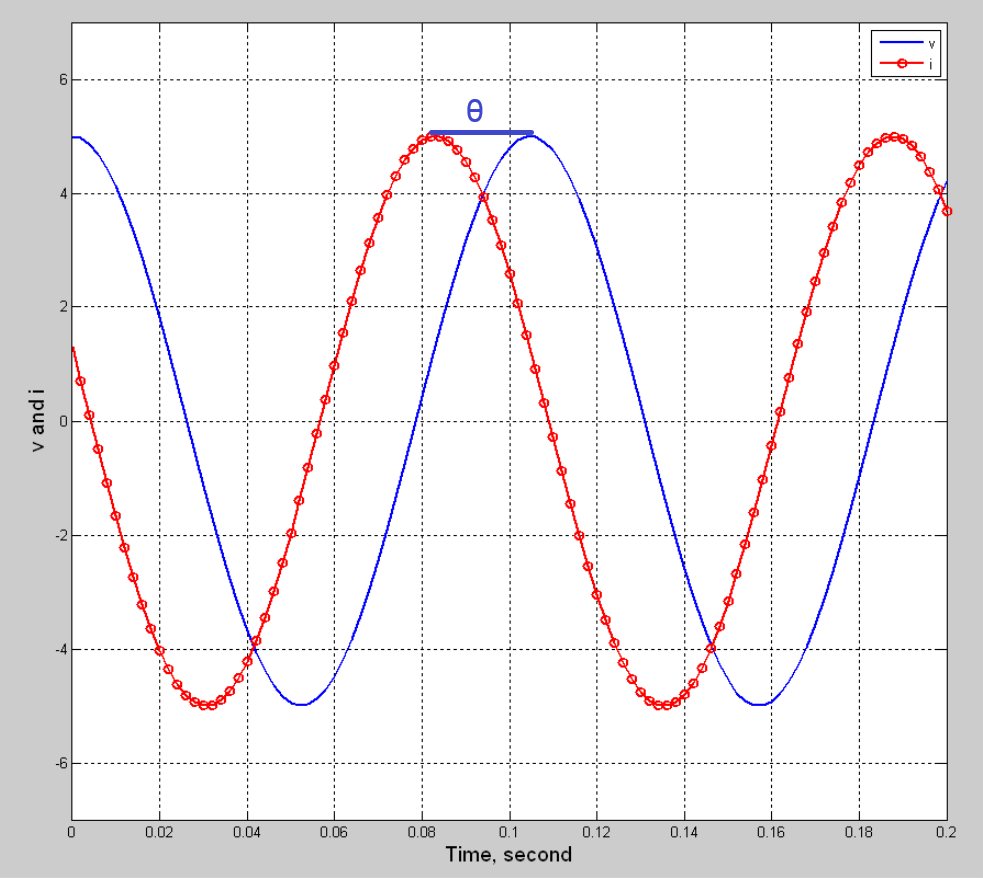
\includegraphics[scale=0.45]{Capture.PNG}
\end{figure}
\subsection{The current i is leading}
\subsection{Per Keysight Infiniivision 2000 X-Series Oscilloscopes User's Guide, measurement of a phase shift between two functions can be obtained, using the oscilloscope, as follow:}

Press the [Meas] Key to display the Measurement Menu, press the Source softkey to select the channel to be measured, press the type softkey and rotate the Entry knob to select phase ans use the setting softkey to select the other channel to measure the phase shift with.

\end{document}